\section{Hydrodynamik - Reale Fluide}

\textbf{Reale Fluide nehmen Scherkräfte auf (Reibung)}

\subsection{Newton'sches Reibungs-Gesetz}
\begin{flushright}
	$\boxed{\textbf{Buch S. 171}}$
\end{flushright}

\subsubsection[Dynamische Viskosität]{Dynamische Viskosität $\eta$}

$$ \boxed{ \tau = \eta \cdot \frac{v}{d} } $$

\renewcommand{\arraystretch}{1.3}
\begin{tabular}{c l c}
    $\tau$                      & Schubspannung                             & $[\tau] = \frac{\newton}{\meter^2}$                                \\
    $\eta$                      & Dynmaische Zähigkeit (Viskosität)         & $[\eta] = \pascal \, \second$                     \\
    $v$                         & Geschwindigkeitsdifferenz zw. Auflagen    & $[v] = \frac{\meter}{\second}$                    \\
    $z$                         & Richtung senkrecht zur Verschiebung       & $[z] = \meter$                                    \\
    $d$                         & Distand zwischen den Auflagen             & $[d] = \meter$                                    \\
    $\frac{\diff v}{\diff z}$   & Geschwindigkeits-Gradient in z-Richtung   & $[\frac{\diff v}{\diff z}] = \frac{1}{\second}$ 
\end{tabular}
\renewcommand{\arraystretch}{1}

\medskip


\para{Werte für $\bm{\eta}$}

\renewcommand{\arraystretch}{1.5}
\begin{tabular}{ll c|c ll}
    $\eta_{\rm Luft}$   & $:= 2 \cdot 10^{-5} \, \pascal \, \second$    & &  $\eta_{\rm Oel}$   & $:= 0.1 \, \pascal \, \second$ \; bis \; $1 \, \pascal \, \second$ \\
    $\eta_{\rm Wasser}$ & $:= 10^{-2} \, \pascal \, \second$            & & \\
\end{tabular}
\renewcommand{\arraystretch}{1}

\medskip


\subsubsection{Kinematische Zähigkeit $\bm{\nu}$}

\begin{minipage}[c]{0.3\columnwidth}
    $$ \boxed{ \nu = \frac{\eta}{\rho} } $$
\end{minipage}
\hfill
\begin{minipage}[c]{0.68\columnwidth}
    \renewcommand{\arraystretch}{1.5}
    \begin{tabular}{c l c}
        $\nu$   & Kinemtaische Zähigkeit    & $[\nu] = \frac{\meter^2}{\second}$    \\
        $\rho$  & Dichte                    & $[\rho] = \frac{\kilogram}{\meter^3}$ \\	
    \end{tabular}
    \renewcommand{\arraystretch}{1.5}
\end{minipage}


\subsection[Stokes'sche Reibung]{Stokes'sche Reibung $\bm{F_R}$}

\begin{flushright}
	$\boxed{\textbf{Buch S. 175}}$
\end{flushright}


Verwendet für z.B. Kugel in Öl

$$ \boxed{ F_R = 6 \cdot \pi \cdot \eta \cdot R \cdot v } $$

\begin{tabular}{c l c}
    $F_R$   & Reibungskraft                     & $[F_R] = \newton$                         \\
    $\eta$  & Dynamische Zähigkeit (Viskosität) & $[\eta] = \mathrm{\pascal \, \second}$    \\
    $R$     & Kugelradius                       & $[R] = \meter$                            \\
    $v$     & Geschwindigkeit                   & $[v] = \frac{\meter}{\second}$		
\end{tabular}


\subsubsection{Kugelfall-Viskosimeter}

\begin{minipage}{0.32\columnwidth}
    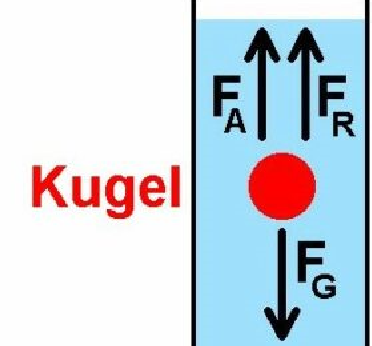
\includegraphics[width=\columnwidth]{images/kugelfall-viskosimeter.png}
\end{minipage}
\hfill
\begin{minipage}{0.6\columnwidth}
    \raggedright

    Auf eine Kugel, welche in einer Flüssigkeit hinabgleitet wirken folgende Kräfte: 

    \medskip

    \begin{tabular}{ll}
        $F_G$   & Gewichtskraft         \\
        $F_A$   & statischer Auftrieb   \\
        $F_R$   & Stokes'sche Reibung
    \end{tabular}

    \medskip

    Ansatz zum Lösen von Aufgaben: \textbf{Kräftegleichgewicht}
\end{minipage}



\subsection{Hagen-Poiseuille}

Beschreibung von \myul{laminaren} Strömungen in einem \myul{runden Rohr} \textrightarrow\ Schichtströmung

\subsubsection{Gesetz von Hagen-Poiseuille}
\begin{flushright}
	$\boxed{\textbf{Buch S. 174}}$
\end{flushright}


$$ \boxed{ V = \frac{\pi \cdot \Delta \, p \cdot t \cdot R^4}{8 \cdot \eta \cdot l} \\ \rightarrow \dot{V} = \frac{\pi \cdot \Delta \, p \cdot R^4}{8 \cdot \eta \cdot l} } $$

\vspace{0.2cm}

\begin{tabular}{c l l}
	$V$ & Volumen & $[V] = \meter^3$ \\
	$\dot{V}$ & Volumenfluss & $[\dot{V}] = \frac{\meter^3 }{\second}$ \\
	$\Delta p$ & Druckdifferenz & $[\Delta p] = \pascal$ \\
	$t$ & dauer des Flusses & $[t] = \second$ \\
	$R$ & Radius des Rohrs & $[R] = \meter$ \\
	$\eta$ & dynamische Viskosität & $[\eta] = \pascal \second$ \\
	$l$ & länge des Rohrs & $[l] = m$ \\
\end{tabular}

\subsubsection{Geschwindigkeitsverteilung von $\bm{r=0}$ bis $\bm{R}$}
\begin{flushright}
	$\boxed{\textbf{Buch S. 173}}$
\end{flushright}


$$ \boxed{ v(r) = \frac{1}{4 \cdot \eta} \cdot \frac{\Delta \, p}{l} \, (R^2 - r^2) } $$

\renewcommand{\arraystretch}{1.3}
\begin{tabular}{c l c}
    $v(r)$                              & Fliessgeschwindigkeit beim Radius $r$ & $[v(r)] = \frac{\meter}{\second}$         \\
    $r$                                 & betrachteter Radius                   & $[r] = \meter$                            \\
    $\eta$                              & Dynamische Zähigkeit (Viskosität)     & $[\eta] = \pascal \, \second$             \\
    $R$                                 & Rohr-(Innen)Radius                    & $[R] = \meter$                            \\
    $\Delta \, p$                       & Druckdifferenz                        & $[\Delta \, p] = \pascal$                 \\
    $l$                                 & Länge des Rohrs                       & $[l] = \meter$
\end{tabular}
\renewcommand{\arraystretch}{1}

\subsection{Ströme mit Reibungen (Turbulent / Laminar)}

\subsubsection{Vorgehen}

\begin{enumerate}
	\item was ist gegeben, je nach dem bereits mit $\Rey$ beginnen
	\item Laminar rechnen (um evt. fehlenden Parameter $\rho, \; v, \; d, \text{ oder } \eta$ zu bestimmen) 
	\item Aus Resultat Reynolds-Zahl $\Rey$ berechnen
	\item Mit kritischer Reynolds-Zahl $\Rey_{\rm kritisch} \le 2320$ vergleichen
	\item Beim \textbf{Überschreiten} \textrightarrow\ Turbulent rechnen
\end{enumerate}
$\rightarrow$ hier bei darauf achten, dass nur weil die Strömung turbulent ist, ein anderes Medium ebenfalls turbulent ist, beispiel kann nur der Überdruck derselbe sein, ohne dessen Reibung zu teilen


\subsubsection{Laminare Strömung}

$$ \boxed{ \Delta p = 32 \cdot \eta \cdot l \cdot \frac{v}{d^2} }  $$


\subsubsection[Überdruck mithilfe]{Überdruck mithilfe $\lambda_x$}

$$ \lambda_{\rm turbulent} = \frac{0.316}{\sqrt[4]{\Rey}}  \qquad \qquad \lambda_{\rm laminar} = \frac{64}{\Rey} $$
$$ \boxed{ \Rightarrow \Delta p_x = \lambda_x \frac{l}{d} \cdot \frac{\rho}{2} \cdot v^2 } $$


\begin{tabular}{c l c}
	$\Delta \, p_x$ & Druckdifferenz (laminar / turbulent)  & $[\Delta p] = \pascal$                \\
	$\eta$          & Dynamische Zähigkeit (Viskosität)     & $[\eta] = \pascal \, \second$         \\
	$l$             & Rohr-Länge                            & $[l] = \meter$                        \\
	$v$             & Fliess-Geschwindigkeit                & $[v] = \frac{\meter}{\second}$        \\
	$d$             & Rohr-Durchmesser                      & $[d] = \meter$                        \\		
	$\rho$          & Dichte des Fluids                     & $[\rho] = \frac{\kilogram}{\meter^3}$ \\
	$\Rey$          & Reynolds-Zahl                         & $[\Rey] = 1$
\end{tabular}


\subsubsection[Reynolds-Zahl]{Reynolds-Zahl $\bm{\Rey}$}
\begin{flushright}
	$\boxed{\textbf{Buch S. 177}}$
\end{flushright}

$$ \boxed{ \Rey = \frac{\Delta \, p}{\tau} = \frac{\rho \cdot \overline{v} \cdot d}{\eta} = \frac{l v}{\text{v}}} \qquad \quad \text{mit } \; \overline{v} = \frac{\dot{V}}{A} , \text{v} = \frac{\eta}{\rho} $$


\begin{tabular}{c l l}
	    $\Rey$     & Reynolds-Zahl                        & $[\Rey] = 1$                               \\
	    $\eta$     & Dynamische Zähigkeit (Viskosität)    & $[\eta] = \pascal \, \second$              \\
	$\overline{v}$ & Mittlere Geschwindigkeit             & $[\overline{v}] = \frac{\meter}{\second}$  \\
	     $d$       & Typische Dimension (Rohrdurchmesser) & $[d] = \meter$                             \\
	$\Delta \, p$  & Druckdifferenz                       & $[\Delta p] = \pascal$                     \\
	    $\tau$     & Schubspannung                        & $[\tau] = \newton$                         \\
	 $\text{v}$  & kinematische Viskosität              & $[\text{v}] = \frac{\meter^2 }{\second}$
\end{tabular}

\medskip

\textbf{Sobald die Reynolds-Zahl $\bm{\Rey}$ grösser ist als ein kritischer Wert bilden sich Wirbel.} \\
\textrightarrow\ Rohr:  $\Rey_{\rm kritisch} \approx 2320$


\subsection{Bernoulli-Gleichung mit innerer Reibung}

\vspace{-0.2cm}

$$ \boxed{ p_1 +  \rho \cdot g \cdot h_1 + \frac{1}{2} \, \crd{\alpha_1} \cdot \rho \cdot v_1^2
= p_2 +  \rho \cdot g \cdot h_2 + \frac{1}{2} \, \crd{\alpha_2} \cdot \rho \cdot v_2^2 \crd{+ \Delta \, p_v} } $$

\renewcommand{\arraystretch}{1.6}
\begin{ctabular}{c| c |c}
                                    & laminar                                                   & turbulent                                                 \\ 
    \hline 
    Korrekturfaktoren               & $\alpha_1 = \alpha_2 = 2$                                 & $\alpha_1 \approx \alpha_2 \approx 1$                     \\ 
    \hline 
    Druckverlust $\Delta \, p_v$    & \multicolumn{2}{c}{$\Delta p_v = \lambda_x \frac{l}{d} \cdot \frac{\rho}{2} \cdot v^2$}                               \\ 
    \hline 
                                    & $\lambda_{\rm laminar} = \frac{64}{\Rey}$                 & $\lambda_{\rm turbulent} = \frac{0.316}{\sqrt[4]{\Rey}}$  \\
\end{ctabular} 
\renewcommand{\arraystretch}{1}

\subsection{Aerodynamik}

Im \cbl{\hyperref[subsec:aerodynamik]{Anhang}} zu finden

\pagebreak

